\documentclass{standalone}
    \usepackage{tikz}
    \begin{document}
    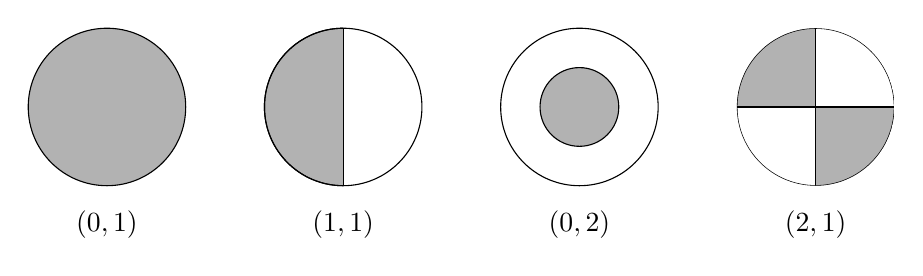
\begin{tikzpicture}
        \draw[fill=gray!60] (0, 0) circle (1cm);
        \node at (0, -1.5) {$(0, 1)$};
        
        \draw [fill=gray!60] (3, 1) arc (90:270:1cm and 1cm);
        \draw (3, 1) -- (3, -1);
        \draw (3, 1) arc (90:-270:1cm and 1cm);
        \node at (3, -1.5) {$(1, 1)$};
        
        \draw (6, 0) circle (1cm);
        \draw [fill=gray!60] (6, 0) circle (0.5cm);
        \node at (6, -1.5) {$(0, 2)$};
        
        \node at (9, -1.5) {$(2, 1)$};
        \clip (9, 0) circle (1cm);
        \begin{scope}
            \fill[gray!60] (8,0) rectangle (9, 1);
            \fill[gray!60] (9,0) rectangle (10, -1);
        \end{scope}
        \draw (9, 0) circle (1cm);
        \draw (9, 1) -- (9, -1);
        \draw (8, 0) -- (10, 0);
        
     \end{tikzpicture}
    \end{document}